\documentclass[tikz,border=5pt]{standalone}
\usepackage{tikz}
\usetikzlibrary{calc}

\begin{document}
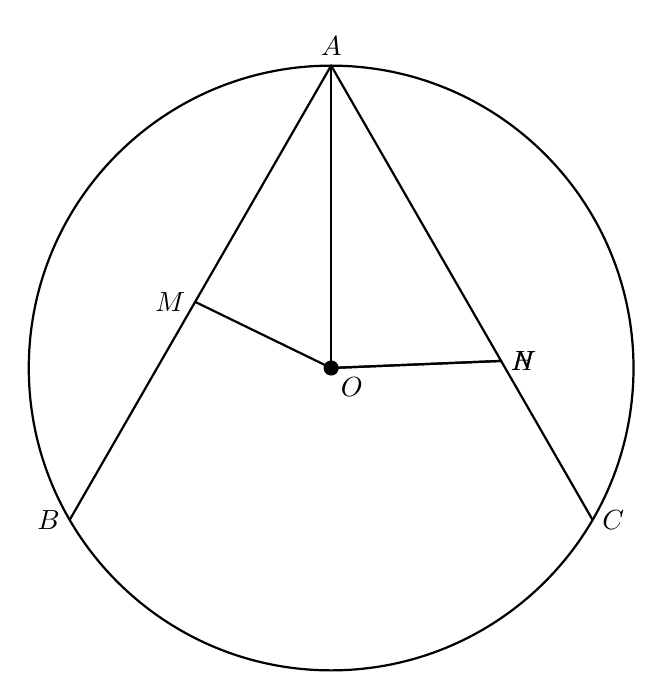
\begin{tikzpicture}[scale=1.2, line cap=round, line join=round]

% Circle and key points
\def\R{3.2}
\coordinate (O) at (0,0);
\coordinate (A) at (0,\R);

% Chords through A
\coordinate (B) at (-2.767,-1.608);
\coordinate (C) at (2.767,-1.608);

% Points on segments
\coordinate (M) at ($(A)!0.52!(B)$);
\coordinate (N) at ($(A)!0.65!(C)$);

% New point H: through O draw line parallel to AB, intersecting AC
\coordinate (H) at ($(A)!0.65!(C)$);

% Circle
\draw[line width=0.8pt] (O) circle (\R);

% Main segments
\draw[line width=0.8pt] (A)--(B);
\draw[line width=0.8pt] (A)--(C);
\draw[line width=0.8pt] (A)--(O);
\draw[line width=0.8pt] (M)--(O);
\draw[line width=0.8pt] (O)--(N);

% Added segment through O parallel to AB
\draw[line width=0.8pt] (O)--(H);

% Point O
\fill (O) circle (0.08);

% Labels
\node[above] at (A) {$A$};
\node[left] at (B) {$B$};
\node[right] at (C) {$C$};
\node[left] at (M) {$M$};
\node[right] at (N) {$N$};
\node[below right] at (O) {$O$};
\node[right] at (H) {$H$};

\end{tikzpicture}
\end{document}
